\documentclass[11pt]{article}
\usepackage[scaled=0.92]{helvet}
\usepackage{geometry}
\geometry{letterpaper,tmargin=1in,bmargin=1in,lmargin=1in,rmargin=1in}
\usepackage[parfill]{parskip} % Activate to begin paragraphs with an empty line rather than an indent %\usepackage{graphicx}
\usepackage{amsmath,amssymb, mathrsfs, dsfont, stackrel}
\usepackage{tabularx}
\usepackage[font=footnotesize,labelfont=bf]{caption}
\usepackage{graphicx}
\usepackage{xcolor}
%\usepackage[linkbordercolor ={1 1 1} ]{hyperref}
%\usepackage[sf]{titlesec}
\usepackage{natbib}
\usepackage{../../Tianpei_Report}
%\usepackage{appendix}
%\usepackage{algorithm}
%\usepackage{algorithmic}

%\renewcommand{\algorithmicrequire}{\textbf{Input:}}
%\renewcommand{\algorithmicensure}{\textbf{Output:}}



\begin{document}
\title{Lecture 3: Randomized Experiments}
\author{ Tianpei Xie}
\date{Sep. 16th., 2022 }
\maketitle
\tableofcontents
\newpage
\allowdisplaybreaks
\section{Randomized Experiments}
\begin{itemize}
\item \emph{\textbf{Randomized experiments}} are noticeably different from \emph{\textbf{observational studies}}.
\begin{itemize}
\item In \emph{randomized experiments}, the experimenter has \textbf{complete control} over the \emph{treatment assignment mechanism} (how treatment is assigned);  Ideally, the treatment assignment is not related to pre-treatment variables, or covariates. 

In randomized experiments, \underline{\emph{\textbf{association is causation}}}. This is because randomized experiments are special in that they guarantee that there is \underline{\textbf{\emph{no confounding}}}.

\item In \emph{observational studies}, the treatment is almost always a function of some covariate(s).
\end{itemize}
\end{itemize}

\section{Association is causation in Randomized Experiments}

\subsection{Comparability and covariate balance}
\begin{itemize}
\item Ideally, the treatment and control groups would be \textbf{the same}, \textbf{in all aspects}, \emph{except for} treatment. This would mean they only differ in the treatment they receive (i.e. they are \emph{\textbf{comparable}}).

\item \begin{definition}(\emph{\textbf{Covariate Balance}}) \citep{neal2020introduction}\\
 We have \underline{\emph{\textbf{covariate balance}}} if the distribution of covariates is the same across treatment groups. More formally,
 \begin{align}
P(X|T=1) &= P(X|T=0)  \label{eqn: cov_balance}
 \end{align} where $X$ is the set of covariates and $T$ is the treatment assignment. 
\end{definition}

\item \underline{\emph{\textbf{Randomization implies covariate balance}}}, across \textbf{all} covariates, \emph{\textbf{even unobserved ones}}. Intuitively, this is because the treatment $T$ is chosen at random, regardless of $X$ i.e. $(T \indep X)$.

\item Under the covariate balance, we can show that $p(y | do(t)) = p(y| t)$, that is, association is causation. 
\begin{proof} 
First, let $X$ be a sufficient adjustment set that potentially contains unobserved variables (randomization also balances unobserved covariates). By back-door adjustment, we have 
\begin{align*}
p(y | \,do(t)) &= \sum_{x}p(y |\, t, x)\,p(x)
\end{align*} Multiplying $\frac{p(t|x)}{p(t|x)}$ we have
\begin{align*}
p(y | \,do(t)) &= \sum_{x}\frac{p(y |\, t, x)\,p(t|x)\,p(x)}{p(t|x)} \\
&= \sum_{x}\frac{p(y, t, x)}{p(t)} \text{ since }T \indep X \\
&= \frac{p(y, t)}{p(t)} = p(y|\,t). \qed
\end{align*}
\end{proof}
\end{itemize}

\subsection{Exchangeability}
\begin{itemize}
\item  \begin{assumption} (\textbf{Ignorability / Exchangeability}) \citep{neal2020introduction}
\begin{align}
(Y(1), Y(0)) \indep T  \label{eqn: Ignorability}
\end{align}
\end{assumption}

\item Exchangeability means that the \textbf{\emph{treatment groups are exchangeable}} in the sense that if they were \textbf{swapped}, the new treatment group would observe the \textbf{same outcomes} as the old treatment group, and the new control group would observe the same outcomes as the old control group. In this sense, our choice of test subjects are nothing special for treatement vs. control. 
\begin{align*}
\E{}{Y(1)} = \E{}{Y(1)\,| T = 0} &= \E{}{Y(1)\,| T = 1} \\
\E{}{Y(0)} = \E{}{Y(0)\,| T = 0} &= \E{}{Y(0)\,| T = 1}
\end{align*}

\item Intuitively, the randomized experiments are exchangeable since we can simply swap the definition of head and tail for the treatment assignment. 
\end{itemize}

\subsection{No backdoor path}
\begin{itemize}
\item The final perspective that we’ll look at to see why association is causation in randomized experiments is that of \emph{graphical causal models}. In regular
observational data, there is almost always confounding. See Figure \ref{fig: random_graph} (Left).
\begin{figure}
\begin{minipage}[t]{0.5\linewidth}
  \centering
  \centerline{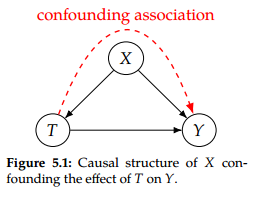
\includegraphics[scale = 0.7]{random_conf_graph.png}}
\end{minipage}
\begin{minipage}[t]{0.5\linewidth}
  \centering
  \centerline{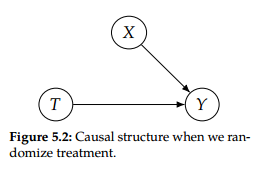
\includegraphics[scale = 0.7]{random_no_back_door.png}}
\end{minipage}
\caption{\footnotesize{\textbf{(Left) Causal structure of $X$ confounding the effect of $T$ on $Y$. (Right) Causal structure when we randomize treatment. \citep{neal2020introduction}}}}
\label{fig: random_graph}
\end{figure}

\item However, if we \emph{\textbf{randomize}} $T$, \textbf{$T$ no longer has any causal parents}.  See Figure \ref{fig: random_graph} (Right). This is because $T$ is
purely random. It doesn’t depend on anything other than the output of a coin toss.

\item Because $T$ has no incoming edges, under randomization, \underline{\emph{\textbf{there are no backdoor paths}}}. So the \textbf{\emph{empty set is a sufficient adjustment set}}. 

This means that \emph{all of the association that flows from $T$ to $Y$ is \textbf{causal}}. Using back-door adjustment for empty adjustment set, we have 
\begin{align*}
P(Y |\, do(T=t)) = P(Y|\, T=t)
\end{align*}
\end{itemize}

\section{Causal Inference in Randomized Experiments}
Under \emph{\textbf{completely randomized experiments}}, association is causation, so \emph{\textbf{causal inference is the same as statistical inference}} and the \underline{\textbf{causal identification}} step is directly completed. We can use hypothesis testing to answer causal questions such as "if treatment has an effect or not". 
\subsection{Hypothesis testing}
\subsubsection{Testing the null hypothesis of no treatment effect}
\subsubsection{Noparametric tests}
\subsection{Attributable effects}
\newpage
\bibliographystyle{plainnat}
\bibliography{book_reference.bib}
\end{document}